\documentclass[twocolumn,10pt]{article}
\usepackage{epsf,verbatim} %,mystyle}
\usepackage{graphicx}

\setlength{\oddsidemargin}{-0.25in}	% 1in from edge of paper
\setlength{\evensidemargin}{-0.25in}	% 1in from edge of paper
\setlength{\textwidth}{7in}		% 
\setlength{\textheight}{9in}
\setlength{\topmargin}{-0.5in} % Top margin at 0.75in
% \renewcommand{\baselinestretch}{1.25}
\renewcommand{\textfraction}{0} 
\renewcommand{\floatpagefraction}{.8}
\columnsep 0.23in

\newcommand{\bib}{bibliography}

% \pagestyle{empty}

\newcommand{\morena}{{MORENA}}

\newcommand{\term}{{\tt terminate}}
\newcommand{\theEnd}{{\tt end}}
\newcommand{\finished}{{\tt finished}}
\newcommand{\start}{{\tt start}}
\newcommand{\fire}{{\tt fire}}
\newcommand{\changedState}{{\tt changed state}}

\newcommand{\termRep}{TERMINATE}
\newcommand{\theEndRep}{END}
\newcommand{\finishedRep}{FINISHED}
\newcommand{\startRep}{START}
\newcommand{\fireRep}{FIRE}
\newcommand{\changedStateRep}{CHANGED_STATE}

\newcommand{\trans}[1]{{\tt transition $<$#1$>$}}
\newcommand{\event}[1]{{\tt #1}}
\newcommand{\elmt}[1]{{\bf #1}}

\newenvironment{note}{\comment}{\endcomment}
\newenvironment{definition}{DEFINITION:}{}
\newenvironment{program}{\verbatim PROGRAM:}{\endverbatim}

\newcommand{\figures}{figures}
\newcommand{\capt}{\caption}
\newcommand{\lang}[1]{{\it #1}}

%\include{extratitle}

\begin{document}

\begin{comment}
  Maybe we should call it PLAINTIF (PLAces, INteractors, TransItions,
  and Flows).  What about PLENTIFUL (PLAces, Transitions, Interactors,
  and FLows)
\end{comment}


\title{\bf The Capoeira\thanks{Capoeira is a Brazilian dance which
    contains elements of a martial art.  It is {\em not} an acronym for
    anything.}\ Model for\\Distributed and Reconfigurable
    Multimedia Systems}

\author{Rodrigo A. Botafogo \\ CAA -- Computa\c{c}\~ao Aplicada \&
  Automa\c{c}\~ao\\ Departamento de Engenharia El\'etrica\\ 
  Universidade Federal Fluminense\\ 24210-240 Niteroi, RJ -- Brazil\\ 
  botafogo@caa.uff.br \and Daniel
  Moss\'e \\ Department of Computer Science \\ University of
  Pittsburgh \\ Pittsburgh, PA 15260\\ mosse@cs.pitt.edu}

\date{}

\maketitle \thispagestyle{empty}

\begin{abstract} 

Recently, a flurry of new multimedia applications, specially CD-ROM
based, have come to the market.  Yet, some statistics show that many
users (upwards of 90\%) consider these multimedia applications to be of
very poor quality.  As with hypertext applications a few years ago, we
can blame that on lack of experience with the new medium, but one of
the most important reasons, in our view, is the lack of good
multimedia authoring tools.

In this paper we propose a flexible yet formal model for developing
distributed and reconfigurable multimedia applications, which takes
into consideration the different types of basic building blocks needed
by users, such as audio, video, text, etc., the user interface,
application customization, synchronization, and also tackles the
scalability and composability problems. We show also our application
builder, based on a Tcl/tk visual tool and discuss briefly how the
applications can be dynamically reconfigured.\\

\end{abstract}


\noindent {\bf Keywords:} {\small Multimedia, distributed systems,
reconfigurable systems, object oriented systems, structured authoring,
  synchronization}

% \footnotetext{
% Permission to copy without fee all or part of this material is 
% granted provided that the copies are not made or distributed for direct commercial 
% advantage, the ACM copyright notice and the title of the publication and 
% its date appear, and notice is given that copyright is by permission of 
% the Association for Computing Machinery. To copy otherwise, or to republish, 
% requires a fee and/or specific permission.

% \copyright 1994 ACM 0-89791-xxx-x/xx/xxxx... 
% }

%\input{introduction}

\section{Introduction}

The advent of new, more powerful, and less expensive computer
technology has made computer users demand that immediate access to
information be more widespread.  The wave of the
``information superhighway'' has led to the development of new
distributed applications, which involve access to diverse types and
forms of data that are geographically dispersed.  The best examples of
these type of applications are the World Wide Web (WWW) and distributed
multimedia (MM) systems.  We are also seeing an increasing integration
of the WWW with MM, in the form of downloadable animation, audio, and
video clips \cite{smi:zeno}.

MM systems have typically been standalone, CD-ROM based, with very
static and well-defined interfaces.  Still, the quality of such
systems falls short of optimal.  In addition, as we approach the third
millennium, we have started observing an escalation in the numbers of
MM systems that require data from different sources, stored across
several sites in a wide-area network (WAN).  For example, customized
news on demand require a combination of videos, charts, maps,
animation, audio, and text.
% Such MM systems are expected to handle
% data streams with equal efficiency and reliability, both from the
% temporal and functional perspectives.
For multimedia digital
datatypes such as video clips, these systems need to synchronize
multiple data streams such as video, audio and possibly superimposed
text.  Thus, in a distributed multi-resource environment, authors must
be able to easily specify the interaction among media and delivery of
several data streams % comprising a single datatype or used in a
                     % single application 
originating at several sources must be performed in a {\em
timely}, {\em synchronized}, and {\em reliable} fashion.

New software technologies, such as CORBA, Object-Orientation, and new
advances in synchronization and real-time in distributed systems, have
enabled progress in the development of distributed multimedia systems.
However, many of these software technologies do not have as their main
concern the authorship or the display abilities that
multimedia systems require.  Therefore, there is an urgent need to
develop specification and modeling approaches that overcome the
current difficulties.

Some recent work on authoring multimedia systems has been described in
the literature.  Some of these are just concerned with the visual user
interfaces for the presentation of multimedia application such as
Escalante \cite{mcw:framework} and some are ad hoc techniques for the
manipulation of different media by users (e.g., showing specific parts
of the media and letting the user zoom in or out, such as Bederson's
zooming web \cite{bed:zoomweb} and Karmouch's VideoTiles
\cite{fal:mmnews}).

In order to compose messages with different types of media that users
can exchange via e-mail, Schirmer and Kirste \cite{sch:mmmail} have
implemented a multimedia mail tool ($M^3$).  Although their interface
for positioning the media on the space reserved for the message is a
good first step, there is little in terms of hierarchical composition
or timing synchronization (from the perspective of media coming from
different sources).  Their tool is built using SafeTCL (concerned with
the isssue of security of data access) \cite{bor:mail}, and incudes a
language for describing the relative positions of objects within a
work area.  Work for doing synchronization of media and their
relative positioning was also done by Ogawa, Harada, and Kameko with
Videobook~\cite{oga:videobook}.

Seminal work has been done in the definition of user interaction
and hypertext navigation by Stotts and Furuta with
Trellis~\cite{sto:tois}.  Our interaction methodology was inspired by
their model and the ease of prototyping is influenced by ideas from
their model structure and simulator.  However, in Petri nets in
general, and in Trellis in particular, synchronization of media is
coarse, i.e., media can only be synchronized at their beginning or
end.  Further attempts at refining Petri net models were done in
OCPN~\cite{lit:ocpn} and its derivations~\cite{qaz:xocpn,pra:aocpn}.

Our preliminary attempt at implementing a model for multimedia
applications resulted in the \morena\ system
\cite{bot:morena,bot:patScenario}.  The \morena\ system was, however,
limited in strength by only providing predefined messages and no data
filtering.  It was also much more limited in the types of
synchronizations it allowed and that its scope was only multimedia
applications.

Our approach differs from the previous ones in that it provides an
environment for multimedia application development taking into
consideration the following issues: structured authoring through a
% DM: WE DON'T USE BIPARTITE ANYMORE. I'M GOING TO SHIP IT THIS WAY
% BECAUSE I DON'T WANT TO CHANGE IT NOW :-)
% IT'S NOT BIPARTITE SINCE THERE ARE FILTERS NOW.  THERE CAN BE
% PLACE -> FILTER -> TRANSITION   AND ALSO % PLACE -> TRANSITION.  QED.
bipartite graph specification, strong (fine) synchronization of
medias, monitoring of data quality and of responsiveness, flexibility
and adaptability through message passing, user interaction, easy
prototyping and simulation (allows use of sketches and does not
require finalized data), a clear model for layout specification (user
interface), and the ability to reuse descriptions through templates (not discussed in this paper further~\cite{tan:scenario}).

Another novelty of this approach is the ability to dynamically change
the presentation by adding and removing places, transitions, flows,
and conditions on them.  This is done based on user input, network
load, and author-specified conditions.

While this authoring tool assumes that resources are plentiful and
will not cause deadline violations, the capoeira model is part of a
larger project dealing with distributed multimedia systems.  The
integration of the Capoeira with the NetWorld
\cite{mos:mmtrafic,mos:mmqos} will allow an author to define and a
system to reliably and timely deliver multimedia data.

The rest of this paper describes the model (Section~\ref{sect-model})
and the language that implements it  (Section~\ref{sect-scripting}).
We describe the status of this project and show our visual tool in
Section~\ref{sect-status} and conclude the paper in
Section~\ref{sect-conc}. 



\section{The Capoeira Model}
\label{sect-model}

The Capoeira model describes a skeleton for the transport and
synchronization of messages through objects in a network, called the
{\em capoeira} network.  The network is composed of the following
elements: {\em places}, {\em filters}, {\em transitions}, {\em
  interactors}, and {\em flows}.  The model also uses a scripting
language to describe the behavior of the components, allowing for easy
reconfigurability and customization.

We will use the term {\em associate} to refer to any of the five
elements of the network, i.e., places, filters, transitions,
interactors, and flows.
A Capoeira net can be defined as a 5-tuple $\langle P, Fi, T, I, Fl
\rangle$, as follows.

\begin{quote}

$P = \{p_1, \ldots, p_i\}$ is a set of {\em places};

$Fi = \{fi_1, \ldots, fi_j\}$ is a set of {\em filters};

$T = \{t_{1}, \ldots, t_{k}\}$ is a set of {\em transitions}; 

$I = \{i_1, \ldots, i_q\}$ is a set of {\em interactors};

$Fl \subseteq \{\langle a_i,a_j\rangle | a_i, a_j \in Fi \cup P \cup
T \cup I\}$ is the set of {\em flow} relations;

\end{quote}

Places are divided in four types: {\em basic}, {\em composite}, {\em
  virtual} and {\em display}.  Filters are divided in two types: {\em
  input} and {\em output}.  Transitions are divided in three types:
{\em input}, {\em output}, and {\em normal}.  Finally, interactors are
divided in two types: {\em basic}, and {\em composite}.

The associates have the following characteristics: 

\begin{itemize}

\item They contain/encapsulate all the information required for proper
  execution.
\item They execute independently having their own thread of execution.
\item They are event driven, in that they are dormant until receiving a
  message, process this message and then return to being dormant.
\item They have an {\em event list}, which contains the events
  they recognize.  When an associate receives a message it recognizes,
  it calls one of its member functions to process the message
  and goes back to sleep.

\end{itemize}


%
% Figures generated with xfig and reduced to 70%
%

\begin{figure}[bt]
    \centering
    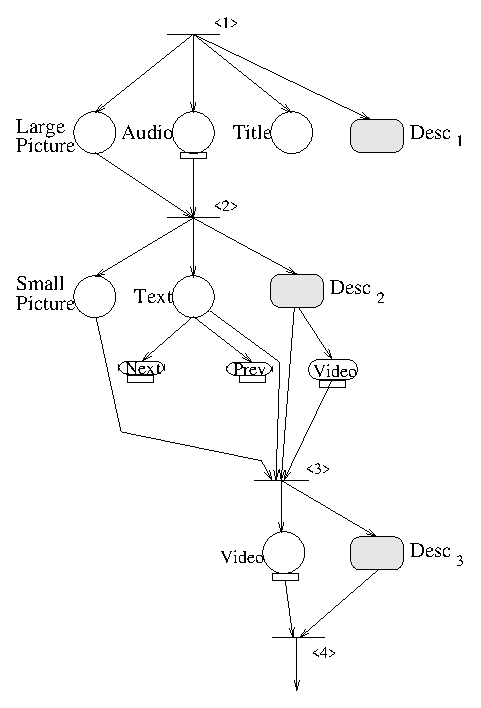
\includegraphics[width=0.4\textheight]{figures/compositePlace.eps}%
    \caption{A composite place made
    of associates: circles represent places, bars represent
    transitions, arrows are flows, ovals depict interactors, and small
    rectangles are filters.}
    \label{fig:compositePlace}
\end{figure}
\textbf{\textit{}}

Figure~\ref{fig:compositePlace} shows a capoeira network with all its
associates.  In all the figures in this paper, basic, composite and
virtual places are represented by circles, while display places are
represented by a shaded, round-cornered square.  This representation indicates that
the first three types of places are in the same class and can be
substituted for each other.  Display places have a different
functionality: instead of being one of the building blocks, they only
define the actual application interface with the users.
Transitions will be represented by bars, interactors by ovals, flows
by directed arrows, and filters by small rectangles attached to any
associate.

\subsection*{Messages}

All the communication between associates is done through message
passing.  A message is a structure composed of the following elements:
{\em Event, Sender ID, Receiver ID, Direction}, and [{\tt Arguments}].

\begin{itemize}
  \item {\em Event}: An event is any command that can be understood by 
        associates, which can
        define to which events they want to recognize.  Examples of events are
        ``MouseUp,'' ``MouseDown,'' \fire, etc.
  \item {\em Sender ID}: The identification number (unique for each associate)
        of the sender.
  \item {\em Receiver ID}: The identification number of the receiver.
        In contrast with the sender ID,  this
        value can be set to NULL, allowing any associate interested in the
        event to receive it.  This is particularly important for message
        distribution and multicasting.
  \item {\em Direction}: The message can be distributed either {\tt
        up} or {\tt down} the hierarchy of places (described below).
  \item {\tt Arguments}: An optional list of arguments.
\end{itemize}

The {\em main} characteristic of a messages is its event.  When no confusion
arises, we will treat the messages and the event in the message
interchangeably.  Therefore, when referring to an event being sent or
received, we are actually referring to the message that carries that
event.


\subsection{Places}

Places are the building blocks of applications, in the sense that they
are the associates that actually perform actions.  For instance,
displaying a video, playing an audio, showing a text, etc.  An application is
constructed by composing places and synchronizing them.

There are four types of places: {\em basic}, {\em composite}, {\em
virtual}, and {\em display}.  Places can be in one of two basic {\em
states}: {\em inactive} and {\em active}.
% It is the responsibility
% of the place to properly store and indicate its state.
A place is inactive only when it is having absolutely no effect in the
execution of the application; otherwise it is active.  
An active place can be in a more specific substate as specified by the
application's designer.  For instance, a video place could
be in the following substates of the active state: running, paused,
fast forwarding, rewinding, and any other substate that the video
place implements.

Every place, basic, composite, virtual, or display, understands a set
of events to which it reacts.  When a place has interest in a message
it has received, it calls one of its member routines to process the
message.  If it has no interest in the message, the place may
redistribute the message to other associates.  % 

An application designer can implement places that understand a variety
of messages but the following two messages must be known by every
place:

\begin{description}
  \item [\startRep] When a \start\ event is received, the place changes
        its state from inactive to active and starts executing.  The
        actual actions to be taken depend on the type of place (basic or
        composite).
  \item [\termRep] When \term\ is received, the place changes its state
        from active to inactive,  cleans all the memory it uses and
        terminates.
        % If the place is a composite place, all its subplaces
        %  are sent the \term\ event.
        % THIS SENTENCE SHOULD ONLY COME AFTER EXPLAINING COMPOSITE PLACES
\end{description}

Although the following two messages must not necessarily be known by
every place, they play an important role in the model.

\begin{description}
  \item [\theEndRep] When a place ends its execution it generates the
        \theEnd\ event.  A continuous media  (e.g., audio, video), for
        instance, would generate the \theEnd\ event when the media it shows
        finishes.  % Note that the place remains active.  
  \item [FINISHED] A place can notify
	other places that it has ended by sending the {\tt finished} event.
\end{description}

\subsubsection*{Basic Places}

A basic place is an executable program treated as a black box by the
model.  The operations or methods it implements and their input
and output values are the sole responsibility of the program (although
they all obey some rules allowing them to communicate with other
associates).  For instance, programs that show a video file, display a
still picture, or send an audio file to the speakers are stored in
basic places.

When a basic place receives a message that is not in its event list it
can either discard it cleanly (i.e., no error is emitted) or it can
generate some error.  In general the messages will be discarded.  This
is equivalent to a window system that discards a mouse click received
outside its active regions.

Basic places can express interest in any type of events.  An audio
place, for instance, might understand the following events:
\event{mute}, \event{speed}, \event{normal\_vol},
\event{lower\_vol}, etc.  Besides those events, it also needs to
understand the two basic events, namely \start\ and \term\ with
the semantics shown above.

% DM: I THINK THAT WE DON'T NEED THESE DEFINITIONS HERE.  IT'S JUST
% DM: REPEATING WHAT WAS SAID LESS THAN A PAGE AGO!!
% \begin{description}
% \item [\startRep] When a \start\ event is received the basic place
%   changes its state from inactive to active and it makes a call to one
%   of its member functions.  An audio place would certainly make a call
%   to the function that starts playing the audio; a video place would
%   certainly make a call to the function that shows the video.
%   However, this is not a requirement.  It is the sole responsibility
%   of the place's developer.
% \item [\termRep] When \term\ is received, the place changes its state
%   from active to inactive, then it cleans all the memory it uses and
%   terminates.  Again, it is the responsibility of the place's developer
%   to guarantee that this function will be properly executed.
% \item [\theEndRep] When the \theEnd\ event is received, the place
%   generates a \finished\ event and sends it outside to be captured by
%   some other associate that might be waiting for this place to end.
% \end{description}
% DM: I also put THE \theEndRep DESCRIPTION above in the generic description

\subsubsection*{Composite Places}

Composite places form complex structures that describe a part of an
application or the
entire application.  Composite places can contain, as
subcomponents, any number or type of associates.

% Composite places
% will be depicted in the figures by a heavy circle.


Note that composite places structure the application hierarchically,
since a composite place can have other composite places inside it.  We
will say that a composite place is the {\em parent} of all the
associates contained within it.  And conversely those associates will
be termed the {\em children} of the composite place.

A composite place can be seen in two levels: {\em imploded composite
place} (ICP), not showing its internal structure, and {\em exploded
composite place} (ECP), in which the subcomponents are shown.  In
Figure~\ref{fig:compositePlace} is one composite place shown in
the ECP view (the whole figure);  \elmt{Video} is in the ICP view (see
Figure~\ref{fig:refinement} for its ECP); the others are basic places.  A
complete application when seen from its highest level is just a single
ICP.  By exploding this view, the next application level is seen.
This process can be continued until all the composite places are in
the ECP view.  Explosion can be done for a single ICP or for all ICPs
inside the ECP.

Keeping places in their ICP view serves the authoring process in two
ways: it hides complexity from the programmer and facilitates
understanding the application's structure.  Also, a composite place in
the ICP view is equivalent to a basic place and thus one can be
substituted for the other.  This functionality can be exploited when
constructing an application by successive refinements.  In a first
prototype of our example application, the video place could be a basic
place showing a video or a still picture.  In a second prototype, we
could substitute the basic video place with a composite video place as
in Figure~\ref{fig:refinement}, which plays two video clips
simultaneously.  This is possible without having to change at all the
description of the whole application.  Rapid prototypes can thus be
made and easily changed reducing the cost of application development.


\begin{figure}[bt]
    \centering
    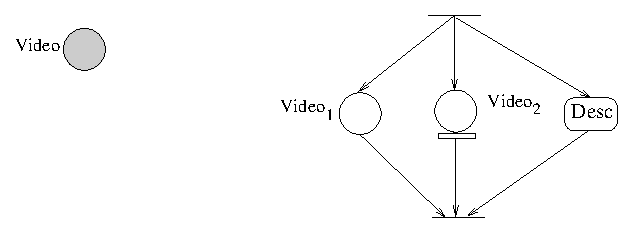
\includegraphics[width=0.4\textheight]{figures/refinement.eps}%
    \caption{The \elmt{Video} place seen in its ICP and ECP views.
            Refinement of the \elmt{Video} place in
            figure~\ref{fig:compositePlace}.}
    \label{fig:refinement}
\end{figure}
\vspace*{-0.5cm}
\textbf{\textit{}}

One should also observe that, due
% In addition to the advantages in program structure,
the hierarchical nature of the structuring of the application,
% allows for
% messages to be distributed among the application associates \cite{}.
% The distribution can be either top-down or bottom-up through the whole
% hierarchy.  The complete distribution rules will be discussed later,
% here it is enough to say that
when a parent sends a message to one of
its children this message can potentially be distributed top-down
until reaching the leaves of the application.  Conversely, when a
child sends a message to its parent this message can be propagated
up, until reaching the root of the application hierarchy.

As with basic places, composite places can also understand any set of
events programmed by the place's developer.  As usual, the two basic
events (\event{start} and \event{terminate}) must be known and
\event{end} is also understood by composite places.  They have the
following additional behavior:

\begin{description}
\item [\startRep] \label{par:start_message} The \event{start} event
      comes in a message with the structure: (\startRep, SID,
      RID/NULL, {\em Direction}
      [{\tt Arguments}]).  An important argument is the {\tt Transition
      Name} (TN) to indicate which of the many possible input
      transitions should fire when the composite place receives the
      \event{start} event.  If no input transition has this name an
      error occurs.
\item [\termRep]  A composite place will first broadcast this event to
      all its children, before terminating as usual.

\item [\theEndRep] \label{par:end_message} A composite place will
      broadcast \term\ events to all its children and will send a \finished\
      event up the hierarchy  (to its parent).
      Note that a composite place that receives the \theEnd\ event does
      not terminate, keeping its memory, execution thread (process), and
      whatever else it needs to proper execution.

\end{description}

If a message other that \start, or \term\ is received, the composite
place's event list is check to see if the place has interest in that
event (the \theEnd\ event is automatically on the event list of
composite places).  If it has, then the
associated member function is called and executed.  If the place has
no interest in that event, the event is broadcast to its parent or all
currently  active children, according to the Direction parameter.

\subsubsection*{Virtual Places}

A virtual place is a place that connects or points (similar to
a symbolic link) to another place that can actually execute.  The
actual place must be aware that it is being used as a {\em surrogate} for a 
virtual place.  Any messages that are received by the actual place and
need to be propagated will be propagated by the virtual place.  In
that sense, the virtual and actual places should be very tightly coupled.

In general the surrogate will be disconnected from other places, that is,
its ICP view has no flows arriving or leaving it.  When a message is
received by the virtual place, it is immediately transferred to the
surrogate (with additional parameters indicating the id of the
virtual place).  When the surrogate finishes execution, any return
value is passed to the virtual place, becoming the virtual's place
return value.

One application of virtual places is for implementing fault tolerance.
They will be used in places where replication is needed.  The virtual
place will pass the event to all replicated surrogates.  However, note
that some places do not allow replication, namely those that perform
input/output operations.  As an example, imagine an automated teller
machine which dispenses money, and in which the task of actually
dispensing the money is duplicated.  The user/customer might be very
happy, yet the bank...

Another implementation of virtual places is to enable transparent
remote execution of places.  For example, if a call is made to a
place, the user need not know whether this is a local C-implemented
routine, or a Remote Procedure Call (RPC) handled by a CORBA object.
This transparency is important when the sources of data are
distributed in geographically dispersed data repositories.

An issue in the execution of a virtual place
is the resource allocation and scheduling
that must occur to guarantee the timely delivery of multimedia data to
the requesting user (see \cite{mos:mmtrafic,mos:mmqos} for more details).


\subsubsection*{Display Places}

Display places are used to describe where
elements of the application will appear on the viewing device (e.g.,
the subtitles appear in the bottom 7\% of the image).
% where the different videos being shown as part of a multimedia
% application will be located on the screen).
A display place is shown in the figures by a shaded round square or
oval.  We will not detail 
the internal implementation of display places in this paper. 
We can use the mechanism in \cite{sch:mmmail} for implementation of
the display place.

A composite place can have many display places, each one giving a
different description of where objects should appear on the screen.
As with the other types of places, display places can either be active
or inactive.  When the display place becomes active, the objects it
describes are shown on the screen at the specified location.  Once the
display place becomes inactive, its description is no longer valid and
the objects are removed from the screen.

It is possible for many display places to be active at the same time,
each one of them describing where some of the objects should appear.
For example, in Figure~\ref{fig:compositePlace}, \elmt{Desc$_1$} is a
display place and it describes where \elmt{Large Picture},
\elmt{Audio} and \elmt{Title} should appear.  \elmt{Desc$_2$}
describes where \elmt{Small Picture} and \elmt{Text} should appear.
Those two description places could be active at once (not in our
example, though).  If two (or more)
display places are active at once and they put the same associate in
two (or more) different places, this associate will be shown multiply.

A natural question is the positioning of overlapping objects.  For
example, if a display place determines that a movie and a picture are
to be located in the same location (or overlapping locations) how can
it be decided which object obfuscates the other?  The relationship
between parent and child places is straightforward: the parent
reserves a specific space on the screen, and such space is used by its
children.  However, in the case of sibling places, the display place
defines the geographic specification of objects on a screen.  That is,
the user will make use of a mechanism as the one proposed in $M^3$
\cite{sch:mmmail}.  If such precedence is not fully specified, the
left-to-right precedence rules will prevail, that is, the sibling that
is mapped onto the screen last will cover the previous
ones. The issue of opaqueness of objects (whether an object is
transparent or not) is currently specified by the users, and its
consequences are to be studied in the future.


\subsection{Filters}

An optional {\em input filter} and an optional {\em output filter} can
be attached to any associate.  A message destined to an associate is
first passed to the associate's input filter, which manipulates the
message as specified by the application builder.  After the input
filter has handled the incoming message, it passes the (possibly
modified) message to the associate for processing.  Analogously, a
message generated by an associate, and sent out from it, first reaches
the output filter and then can continue its way following the message
distribution rules.  The output filter has similar functionality as
the input filter.

Among the possible functions of the input and output filters are:
strong type checking, checking the validity of the message,
changing the contents to ensure proper/faster processing, stripping
headers, delaying the delivery to ensure proper ordering of messages
or proper resource utilization, or simply omitting to forward the
message to the destination place.

An input filter can also be used to force the execution of an
associate's member routines.  Suppose for instance that an
initialization routine is to be executed every time a place receives
the \event{start} message.  The input filter would receive the message,
call the initialization routine, and only then send the
\event{start} message (with possibly modified parameters) to the
place.

In addition to the input filter functionality, output filters have a
very important function in the model: it is through them that
conditional and/or parameterized branching is possible.  Remember that
when a message is generated by an associate, it first reaches the
output filter.  Based on that message the filter can chose to which
associate and which message to send.  We have shown elsewhere that
such property (called {\em functional polymorphism}\footnote{The
concept is similar to discretely adjustable media
segments~\cite{buc:tempLayout}.  The difference is that we deal with
functions and in \cite{buc:tempLayout} the {\em actual data} may have distinct
representations and different durations.}) is very powerful and
allows not only for dynamic behavior of applications, but also for
fault tolerance \cite{mos:obrt}.

In the figures we represent filters by small rectangles attached to
the associates.  In Figure~\ref{fig:compositePlace} there are five
output filters: one attached to place \elmt{Audio}, one to place
\elmt{Video}, and three others attached to each interactor.

For example, if a place processes the data (say in MPEG format) and
needs to send it to another place which does not understand the same
format (say it understands only MotionJPEG format), a filter can be
used to marshall and unmarshall the data.  This is
the same principle used by RPC stubs, but can also be
used for checking the validity of data being generated by a place.

\subsection{Transitions}

The functionality of transitions in this model is similar to that of
transitions in a Petri Net, since it functions as a synchronization
agent, which transitions the program from one state to another.  For
example, they are responsible for
starting and ending execution of places.  They can be used to ensure
that a set of places has reached a certain state before continuing the
application's execution.


We now define the preset
and the postset of a place, transition, or interactor.  The term {\em
node} will be used to refer to any of those three elements.\\

\begin{definition}
  Let $Fl$ be the set of all flows.  The preset and postset of a node
  $n_i$ are defined respectively as:
  \[\bullet n_i = \{n_j\ |\ \langle n_j,n_i \rangle \in Fl\},\]
  \[n_i \bullet = \{n_j\ |\ \langle n_i,n_j \rangle \in Fl\}.\]
\end{definition}

Transitions can be of three types: {\em input}, {\em output}, and {\em
normal}.  An input transition has no preset, while an output
transition has no postset.  Normal transitions have both non-empty
preset and postset.  Transitions will be depicted in the figures by
horizontal bars.  Every composite place needs to have at least one
{\em input transition} but it can have as many as desired by the
application author.  In general, composite places also have one or
more {\em output transitions}.  In Figure~\ref{fig:compositePlace},
\trans{1} is the only input transition while \trans{4} is the only
output transition.


A transition can be in one of two states: {\em active} and {\em
inactive}.  Input transitions become active when the embedding
composite place to which they belong (their parent) starts execution.
In other words, when a composite place receives a \event{start}
message, all its input transitions become active.  On the other hand,
for normal and output transitions to become active, it is required
that an {\em activation set} (AS) of said transition becomes active.\\

\begin{definition}
  An {\em activation set} of a transition $t$ is a pre-defined subset
  of the preset of $t$.  An activation set is said to be {\em active}
  if all its places are in a state specified by $t$.
\end{definition}

For example, let $P_i$:$\langle state\rangle$ be a place in the preset of $t$
that is in the given substate of the active state.  Then $S_1 =
\{P_1:normal, P_2:ready, P_4\}$ and $S_2 = \{P_2:ready, P_3, P_4\}$
could be two activation sets.  If during the application's execution,
place $P_1$ is in a normal state, $P_2$ is ready, and $P_4$ is active,
then $S_1$ would be active.  If $P_3$ is also active, then both $S_1$
and $S_2$ would be active.

To simplify its interface, a transition may receive messages from any of
the places in its pre-set.  Transitions need to recognize only two types of
messages: \event{fire} and \event{changed state}.  The latter type of
message is received and processed by either an active or inactive
transition, but \event{fire} messages will be simply discarded by inactive
transitions.

On the other hand, an active transition will activate a {\em script} when it
receives a \event{fire} message.  A transition  script consists
of $\langle${\em place, event}$\rangle$ pairs which determine a set of
places in its preset and postset to which messages should be sent when
the transition fires.  For instance, the following is a typical transition
script: \{sendPre(\termRep); sendPost(\startRep)\}, which will
send \term\ events to all the places in the transition's preset and
\start\ events to the places in its postset.

When a place in the transition's preset changes state, it sends to the
transition the \changedState\ message, with an argument indicating its
new state.  This value will be used to check if any of the
transition's activation sets has become active.

\subsubsection*{Input Transitions}

Input transitions are used to start the execution of composite
places, and thus every composite place needs to have at least one input
transition, although there can be more than one.  When a composite place is to
be executed, a \start\ message is sent to it and depending on the
\start\ parameters an associated input transition fires.  Since input
transitions have no preset, they become active as soon as the
composite place containing them becomes active.

Recall from Section~\ref{par:start_message} that the \start\ message
has the form: (\startRep, SID, RID/NULL, {\em Direction}
[{\tt Arguments}]).
Every input transition has a unique {\em signature} composed of SID, RID, and
{\tt Argument Types} (optional).  Two input transitions cannot have
the same signature.  When a \start\ message is sent to a composite
place, IDs and {\tt Arguments} are compared with the transition's
signature.  If there is a match, this transition will be sent a \fire\
message with the given arguments.

\subsubsection*{Normal Transitions}

Normal transitions are transitions with preset and postset.  They are
used to synchronize the execution of the application.  They typically
process  \changedState\ messages and wait for a \fire\ message to
be sent to them.  When this message is received and the transition is
active, it sends messages through its flows as its script dictates.

For example, assume that \trans{2} in Figure~\ref{fig:compositePlace}
has the following script: \{sendPre(\termRep);
sendPost(\startRep)\}.  When this transition fires it will send to
its preset the \event{terminate} message ending the places:
\elmt{Large Picture} and \elmt{Audio}.  It will also send
\event{start} messages to its postset.  This will start the places:
\elmt{Small Picture} and \elmt{Text}; and will show them on the screen
following \elmt{Desc$_2$}.


\subsubsection*{Output Transitions}

Composite places can have zero or more output transitions.  Output
transitions can in a sense be compared to return statements in C.
When an output transition fires it notifies (through message passing)
its parent of the successful completion of its (the parent's) task.
This notification is done by sending an \theEnd\ message.  If an error
has occurred, the transition will still fire and the output filter at
the parent's place will catch/handle the error.
% REPEATING IT.
% of the form:
% (\theEndRep, SID, RID, [{\tt Arguments}]), where SID is the output
% transition's ID, RID is the parent's ID and {\tt Arguments} are the
% optional arguments.  Section~\ref{par:end_message} describes the
% actions taken by a composite place when the \theEnd\ message is
% received.

Note that if a composite place has no output transition, it cannot
notify the exterior world of its ending.  This will generally be the case
for non-continuous media, such as text, still pictures, etc, since
they produce no effect on the outside world.  These
places will be terminated by an external associate, not internally.



\subsection{Interactors}

Interaction between the user and the application is done through the
use of {\em interactors}.  Such interaction may consist of
button-pressing commands, resizing, pausing, and other commands a user
may issue to the application.  Interactors can be of two types: {\em
  basic}, and {\em composite}.  Interactors are in some sense a mix
between transitions and places.  As transitions, they become active
when one of its activation sets becomes active.  As places, they can
be composite, and they are composed of any number of associates.

Interactors also understand messages that are sent to them.  Since
they are the intermediaries between user and application, either the
application or users can send messages to the interactors.  However, some
restrictions apply\footnote{We may want to call this the {\em modified
advertisement rule}, since we say that ``some restrictions apply'',
but do not limit it to users that are 18 or older, and do not add
sales taxes where applicable.}:  the only
message all interactors understand is the \changedState\  
message and basic interactors can also receive messages from
outside the network, i.e., coming from the user.

Analogous to transitions, an inactive interactor can only express
interest in the \changedState\ message.  Only when the interactor
becomes active, can it express interest in user events.  If the
interactor becomes inactive again, it is forced to drop its
interest in user events.

\subsubsection*{Basic Interactors}

Basic interactors are system dependent.  They read input from the user
according to the system's specification.  For instance, if the model
is implemented on top of X-Windows, then basic interactors will
receive X-events such as {\em KeyPress}, {\em KeyRelease}, {\em
ButtonPress}, etc.  This can be implemented by setting the
appropriate event masks.

Basic interactors can also receive simulated user interaction events
comming from the network.  For instance, it is possible to have a
timer place send a simulated user click on a button if the button is
not pressed within a time interval from its activation.

\subsubsection*{Composite Interactors}

A composite interactor is a complex structure that can be specified
using the same rules as composite places, except that it can have one
and only one input transition.  This input transition fires when the
interactor becomes active.

Figure~\ref{fig:compositeInteractor} shows a composite interactor that
acts as a button.  First let's look at its ECP view 
% DM: THERE IS NO RIGHT OR LEFT SIDE IN THIS FIGURE.
% on the right side of
IN Figure~\ref{fig:compositeInteractor}: It has a
visualization (BV), that changes its representation depending on
whether the mouse is inside or outside the button.  When the
interactor becomes active, BV is in a normal state.  MI, MO, and DC
are basic interactors that track the mouse, the first checking if the
mouse is inside the button area, the second if the mouse moved outside
of the button, and the third if the mouse has been double clicked.
MI's activation set is {\em BV:Normal}, indicating that MI will
become active when BV is in the Normal state.  The activation set for
MO and DC is {\em BV:Ready}.  When the mouse gets inside the button
area MI sends a message to BV so that it changes its state to Ready
and shows it visually.  At that moment MO and DC become active and MI
inactive.  If the mouse gets out of the button area, MO sends a
message to BV so that it again becomes Normal.  If DC finds that the
mouse has been double clicked it fires the output transition, which
sends an \theEnd\ message to the button (not represented).

% When the \theEnd\ message is sent it is captured by the button's
% output filter.  Now, on the ICP view (left side of
% Figure~\ref{fig:compositeInteractor}), we can see that the interactor
% is connected to two transitions.  The filter can at this point send
% different or the same messages to each one of those transitions.  It
% could, for example, send \event{fire} messages to both of them, which
% would start the two places concurrently.


\begin{figure}[bt]
    \centering
    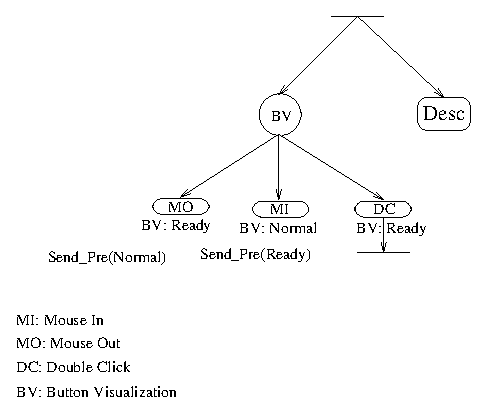
\includegraphics{figures/compositeInteractor.eps}%
    \caption{The \elmt{NEXT} composite interactor seen in its ECP view.}
    \label{fig:compositeInteractor}
\end{figure}
\vspace*{-0.5cm}
\textbf{\textit{}}

\subsection{Flows}

Inside a composite place, {\em flows} are used to connect the
different associates.  The following are possible connections (for
flows, places/interactors represent their input and output filters):
%
\begin{itemize}
\parskip 0pt
\item Place to Transition
\item Place to Interactor
\item Transition to Place
\item Interactor to Place
\end{itemize}
%

Flows are the ducts through which messages are sent.  They connect the
many associates in the application and can also be used for aiding
transparent remote operations of virtual places.  That is, the user or the application
designer need not be cognizant of the location of the tasks to be
executed.

When one of the associates wants to send a message, it passes this
message to the appropriate flow (this is automatic, without user
intervention).  For example, when \trans{2} in
Figure~\ref{fig:compositePlace} sends a sendPost(\startRep) message,
this message is given to the three out flows connected to it: leading to
\elmt{Small Picture}, \elmt{Text} and \elmt{Desc$_2$}.

Each flow knows the location of its source and destination, that is,
in which host they are executing.  Having the message to be send, they
convert it to an appropriate format and send it using a particular
protocol.  Each flow could use a different communication protocol.
For instance, our sendPost(\startRep) message could be converted to:
sendPost(\startRep, Host:SenderID, Host:ReceiverID, nullDirection, [{\tt Arguments}].
% DM:  I removed the following sentence, it has nothing to do.
% The communication protocol used by the first two links could be
% TCP/IP, while the third link uses an ATM protocol.

%DM: I added the following.
This powerful abstraction makes the issue
of resource allocation at the network level orthogonal to the design
of the application.  We note, however, that distributed multimedia
applications will require high bandwidth, which will probably be
present in ATM-based network.  If reservations of links are required
by the application and/or user, the capoeira model can request the
services of a network reservation algorithm such as those proposed in
\cite{fie:vnet,fer:rtchannel}.

\section{Scripting Language}
\label{sect-scripting}

The Capoeira model can be strongly customized based on scripts that
execute when messages are received or upon the occurrence of events.  In
addition to the typical features (e.g., loops, function calls,
variables, etc), our language also has special functions that are
cognizant of the structure of the model and with which the whole
functioning of the model can be changed.  In this section we will show
how a multimedia development tool can easily be implemented on top of
Capoeira by writing scripts for each associate.

In order to make our explanations more concrete, they will be based on
Figure~\ref{fig:compositePlace} that shows an example of a multimedia
application specified using the capoeira model.  As we explain the
model, we will refer to the figure and show how it implements the
application specification given below.

\subsection*{First Application}

What we see in Figure~\ref{fig:compositePlace} is actually only the
introduction to an application.  When this application starts, the
title of the application, a large picture, and an audio start playing.
The title should stay on during the whole application.  

When the audio ends, the large picture disapears and a small picture
and a text appear.  Also, three buttons labeled \elmt{Next},
\elmt{Prev} and \elmt{Video} will appear.  If the user presses the
\elmt{Next} or \elmt{Prev} buttons, the text will change pages
accordingly.  When the \elmt{Video} button is pressed the picture,
text, and buttons all disappear, and a video starts playing.  When the
video ends, the introduction is over.

Our main synchronizing agents are transitions and changing their
script has the most impact over the application.  The following script
functions are stored in a library for use in transitions:
\lang{sendPre}, \lang{sendPost}, 
\lang{send}, \lang{sendAAS}, and \lang{sendParent}.  The first two,
namely \lang{sendPre}
and \lang{sendPost}, send a message to the preset and postset,
respectively.  \lang{send} sends a message through a specified flow,
\lang{sendAAS} sends a message to all active members of activation
sets, and \lang{sendParent} sends a message to the parent (if there is
one).

For a multimedia system, the following could be the scripts for the
input, output and normal transitions:

\small

\begin{program}
Input Transitions:           
On FIRE {                    
  sendPost("START");         
}                            
                         
Normal Transitions:     
On FIRE {               
  sendPre("TERMINATE"); 
  sendPost("START");    
}                       

Output Transitions: 
On FIRE {           
  sendPre("TERMINATE"); 
  sendParent("FINISHED");
}                   

\end{program}
\normalsize

In our example of Figure~\ref{fig:compositePlace}, when the
application starts, its unique input transition (\trans{1}) fires.
This is so since in the model an input transition becomes active as
soon as its parent becomes active and also because when an application
starts it sends a fire to the input transition of the root associate
(passing to it command line arguments).  When it fires, it executes
the {\tt InputTransition}'s script, which sends to its postset the
\start\ message, starting simultaneously the Large Picture, the Audio,
the Title, and showing them simultaneously on the screen following the
description given in the display place $Desc_1$.

Let us assume that  every active place in the preset of a normal
transition is an activation set for that
transition.  In that case, \trans{2} becomes active as soon as the
Large Picture or the Audio becomes active.  When the Audio ends, it
sends a \finished\ message up the hierarchy.  Let us set the filter
script associated with the audio to:

\small

% DM: SHOULD THIS BE  on END???
\begin{program}
On FINISHED {
  sendPost("FIRE");
}
\end{program}

\normalsize

A \fire\ message is then sent to \trans{2}.  This transition executes
the {\tt NormalTransition}'s script, which sends to the preset \term\
messages and to the postset \start\ messages.  This removes the Large
Picture from the screen, frees associated memory from the picture and
audio, and starts the Small Picture and Text.  Note that the Title is
unaffected, satisfying our application's specification. 

Let us now consider the user's interaction with the application
through the video interactor.  We would like it to perform like a
button: when the user presses it, we want the Video Place to start
execution.  When this interactor becomes active, it starts tracking
the mouse as described in the previous section.  When the mouse is
clicked it sends a \finished\ message, which is caught by the filter.
This filter sends a \fire\ message to
\trans{3}.  This, in turn, will remove the Small Picture, the Text
(along with its subordinate interactors), and start the Video Place.
(Note that the display place ending will make the video interactor be
removed from the screen.)

When the Video ends, again a \finished\ message is sent.  It will be
caught by the filter, firing \trans{4} which sends an \theEnd\ to its
parent (the application).  The application then sends a \term\ to all
its children and dies.  At this point, the Title is erased.

The other two associates of interest are the filters connected to the
\lang{Next} and \lang{Prev} interactors.  The following could be the
scripts associate with them.

\small

\begin{program}
'Next' Filter:             'Prev' Filter:
On END {                   On END {                  
  sendPre("NEXT_PAGE");      sendPre("PREV_PAGE");   
}                          }                         
\end{program}

\normalsize

Note that the preset and postset of a filter is the same as the preset
and postset of the associate to which they are connected.


\subsection*{Second Application}

Consider now a slight change in our application.  Assume that the Audio is
describing in some way the scene shown in Large Picture.  When the
Audio makes a reference to a
particular feature of the Picture, we want that feature to be
highlighted.  For that, assume that there is a mark in the
audio so that whenever this mark is reached a message "FEATURE $i$"
is sent up the hierarchy, where $i$ is the number of the feature we want
highlighted.  Assume also that the flow between the Large Picture and
\trans{2} is labeled 1.  We change the filter's script as follows:

\small

\begin{program}                    
On FEATURE {                 On FINISHED {      
  sendPost(<HIGHLIGHT,i>);     sendPost("FIRE");
}                            }                  
\end{program}

\normalsize

And \trans{2} script becomes:

\small

\begin{program}
On HIGHLIGHT {              On FIRE {                   
  send(<HIGHLIGHT,i>, 1);     sendPre("TERMINATE");     
}                             sendPost("START");        
                            }                           
\end{program}

\normalsize

The function \lang{send($\langle$HIGHLIGHT, i$\rangle$, 1)} sends the
message \lang{$\langle$HIGHLIGHT, i$\rangle$} through flow 1.  When the place
receives this message, it will highlight the specified feature.

Note that inter stream synchronization is obtained by a simple change
in scripts.  Although this change was a slight one,  note that the 
mechanism is very powerful, since
more radical changes can alter greatly the execution.

The
scripts shown above should be part of a standard multimedia
distribution.  Other systems, such as general distributed
applications or digital signal processing, would have customized
scripts implemented as a permanent library offered to users.

\section{Status}
\label{sect-status}

Our initial implementation of the model was developed using Tcl/tk and C++.
We use Tcl as the base for our scripting language to which we added
the functions particular to the model.  The runtime system is
interpreted and based on the automaton extracted from the
model.
We also use Tcl/tk for the implementation of the user interface, both
during runtime and during the authoring process.  Our display places
are Tcl/tk scripts specifying the position of the diferent medias on
the screen.

Figure~\ref{fig-capoeira-prot} on page~\pageref{fig-capoeira-prot} shows a capoeira net being created
using our authoring tool.  This preliminary editor allows an author to
create the presentation by adding the different types of basic places
(audio, video, text, picture, display), and enables saving/loading of
applications for completion and modification.  The output of this
editor is an executable specification (the automaton description).

The individual node editors allow the author of the multimedia
application to enter different specific details for each type of basic
building block.  In the figure we can see that the node editor on the
bottom left is for a ``vplace'' (or {\em video} place) and requires
the name of the file where the video is stored, the duration and play
rate of the video, and also the size of the video on the screen.  The
size, however, is not a required field and there is no guarantee that
this size will be the actual one during execution.  This value is just
a prefered size.

The node editor on the bottom right is for a picture place (pplace),
and does not require the duration or play rate.  Thus only the
relevant fields are shown.  Similarly, the audio place would not need
a play rate, and the text place would require only file name and size.

\begin{note}
RB:  Not clear at all for me.

Note that the place's characteristics are determined by the author
(much the same as the director of a movie or a playright), but during
playback users may change these characteristics (e.g., quicktime
videos).
\end{note}

\section{Conclusion}
\label{sect-conc}

We have shown a system for structured authoring of multimedia
applications, and have shown the visual tool that aids such process.
The powerful message distribution mechanism, and the basic building
blocks for multimedia applications make use of message passing, and
allows developers to use it synchronously or asynchronously.

The strong synchronization of media, and their positioning and display
on the limited screen space, is coordinated by the author of the
application.  The synchronization can be changed without changing the
structure of the application, but simply changing the scripts.
Further, the possibility of statically or dynamically changing the
application (serving the purposes of application refinement and
on-the-fly functional polymorphism) is an integral part of the model.

In addition, our system allows for monitoring of data quality and of
responsiveness through filters, flexibility and adaptability through
message passing up or down the hierarchy of composite associates,
well-defined user interaction through special interactor icons, easy
prototyping and simulation (allows use of sketches, and does not
require finalized data) through virtual places, and a clear model for
layout specification (user interface) via display places.

Even though we have not elaborated on the following issues (future
work), we have left placeholders in the model for their insertion in
the model.  We intend to focus on different fronts, as follows.
\begin{itemize}
  \item The addition of fault tolerance capabilities to the model
        (according to the user's specification but without forcing the
        user to determine the fault-tolerant policies to be used).
  \item The resource allocation and scheduling issues, integrating the
        Capoeira model with the NetWorld system
        \cite{mos:mmtrafic}, to obtain an
        comprehensive and cohesive environment for the development and
        deployment of distributed multimedia applications.
\end{itemize}
  
Lastly, the prototype implementation using Tcl/tk is portable and can
be used in a variety of environments.  Since this model is based on a
Petri-net framework, it is highly executable and easy to implement.

\small

\bibliography{\bib/misc,\bib/hypermedia,\bib/distributed}
\bibliographystyle{plain}

\onecolumn

\begin{figure}[bt]
    \centering
    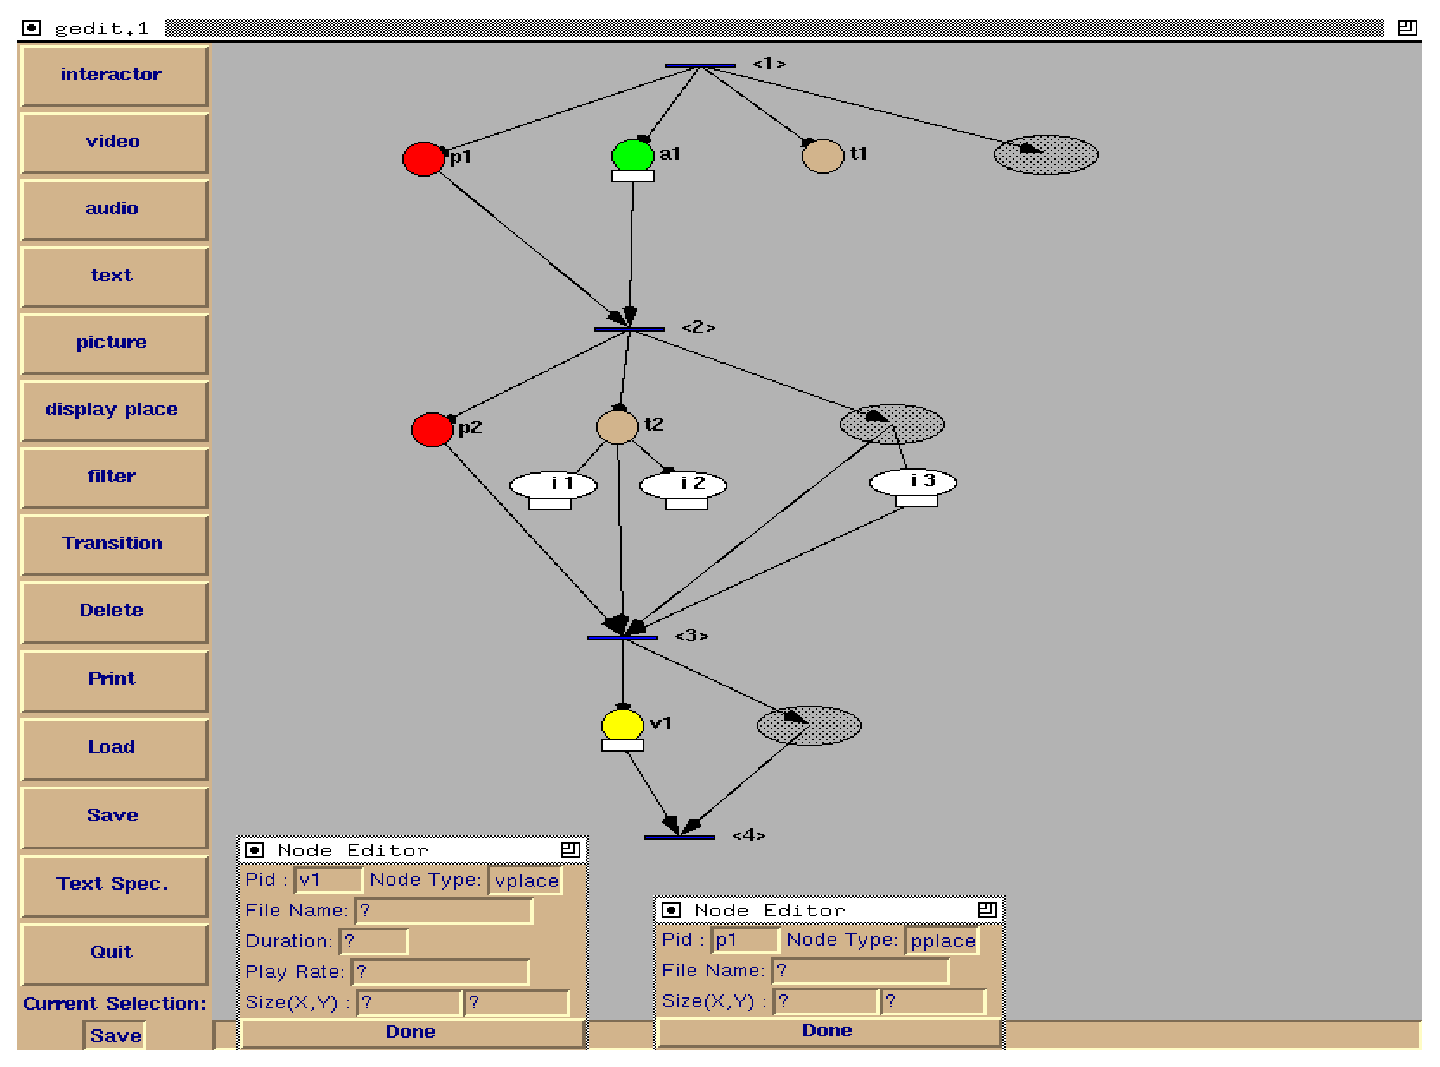
\includegraphics[width=0.8\textheight]{figures/capoeira-prot.eps}%
    \caption{The Capoeira author interface.  Note that the specific details
of each media are given in a node editor (two of them, for 
video and still picture are shown at the bottom of the figure).}
    \label{fig-capoeira-prot}
\end{figure}
\vspace*{-0.5cm}
\textbf{\textit{}}

\end{document}
